\fancyhead[L]{CAPITOLO 3}
\fancyhead[C]{}
\section{Creazione del dataset}
Dall’analisi effettuata nel capitolo precedente sono emerse diverse criticità nello studio dei \emph{flaky test}. Tali criticità sono sinonimo di un argomento di ricerca ancora molto da approfondire. Le problematiche maggiori che sono state sono evidenziate all’interno della ricerca sono principalmente legate alla carenza di dati
messi a disposizione per la comunità. Infatti, in molti degli studi precedentemente analizzati, la carenza di dati viene considerata una minaccia alla validità poiché i progetti considerati sono quasi tutti scritti in linguaggio \textbf{Java} ed usano \textbf{Maven} come
sistema di building. Avere diverse tipologie di dataset risulta estremamente importante in quanto tale problematica risulta ancora di notevole interesse da parte delle grandi multinazionali che ogni giorno sviluppano centinaia di progetti utilizzando differenti linguaggi di programmazione.

Nel 2019, nell’ambito della conferenza “\emph{Testing and Verification Symposium}” organizzata da Facebook, sono stati proposte diverse idee innovative che potessero in qualche modo far fronte alla problematica flakiness. Tra le idee
maggiormente apprezzate è possibile citare: “\emph{A scalable infrastructure for fuzzy-driven root causing of flaky tests}” ideato da Filomena Ferrucci (Università di Salerno), Pasquale Salza (Università di Zurigo) e Valerio Terragni (Università della
Svizzera italiana).

La loro idea prevede un nuovo approccio per identificare le \emph{root cause} di un \emph{flaky test}, che non prevede nessun tipo di “\emph{instrumentation}” del codice, ma va ad
identificare la \emph{root cause} dei flaky test, eseguendo il caso di test in differenti configurazioni definite da cluster. Ogni cluster esplora attivamente uno specifico
spazio di esecuzione \textbf{non deterministico}. Il cluster che mostrerà i risultati più
bilanciati tra “pass” e “fail” sarà utilizzato per identificare la root cause di quello
specifico \emph{flaky test}. Il primo passo da fare per sviluppare questo nuovo tool è creare un nuovo dataset con quanti più \textbf{flaky} test possibili.\cite{Container}
\section{Approccio alla problematica}
L’idea di base è stata quella di partire da un dataset già esistente, ossia quello
rilasciato dagli sviluppatori di \textbf{iDFlakies}, ed ampliarlo con nuove informazioni.
Questo framework, rilasciato nel 2019 permette l’individuazione di un \emph{flaky test} con una classificazione parziale (dipendente dall’ordine e indipendente dall’ordine).

Il dataset rilasciato con questo framework conta al suo interno
quattrocentoventidue \emph{flaky test}, di cui il 50.5\% sono dipendenti dall’ordine, mentre i restanti 49.5\% sono non dipendenti dall’ordine.
L’individuazione dei \emph{flaky test} all’interno del tool di \textbf{iDFlakies} avviene tramite una serie di configurazioni che cambiano l’ordine di esecuzione sia delle classi di test che dei test case al loro interno.
Tra le configurazioni presenti all’interno di \textbf{iDFlakies}, possiamo citare:
\begin{itemize}
	\item \emph{Original-order}: Esegue tutti i casi di test nell’ordine in cui sono stati scritti
	dallo sviluppatore;
	\item \emph{Random-Class}: Esegue le classi della suite di test in ordine pseudo-casuale, ma mantenendo l’ordine originale di esecuzione dei test all’interno di ogni classe;
	\item \emph{Random-class-method}: Esegue gerarchicamente prima in ordine pseudo-casuale le classi che compongono la test suite per poi eseguire in maniera pseudo-casuale i singoli casi di test che compongono le varie classi;
	\item \emph{Reverse-class}: Inverte l’ordine di esecuzione delle classi di test ma mantiene invariato l’ordine di esecuzione dei singoli test all’interno della classe;
	\item \emph{Reverse-class-method}: Inverte l’ordine sia delle classi di test che dei metodi di test al suo interno.
\end{itemize}

Analizzando il dataset messo a disposizione è emerso che ogni progetto contiene le informazioni presentate nella tabella sottostante:
\begin{table}[h]
	\centering
	\scalebox{0.8}{
	\begin{tabular}{|l|l|l|l|l|l|l|}
		\hline
		\textbf{URL} & \textbf{SHA} & \textbf{Test count} & \textbf{Module Name} & \textbf{Test Name} & \textbf{Category} & \textbf{Version} \\ \hline
	\end{tabular}}
\end{table}
La figura \ref{fig:datasetRilasciato} mostra un esempio per descrivere il contenuto del dataset
rilasciato.
\newpage
\begin{figure}[h]
	\centering
	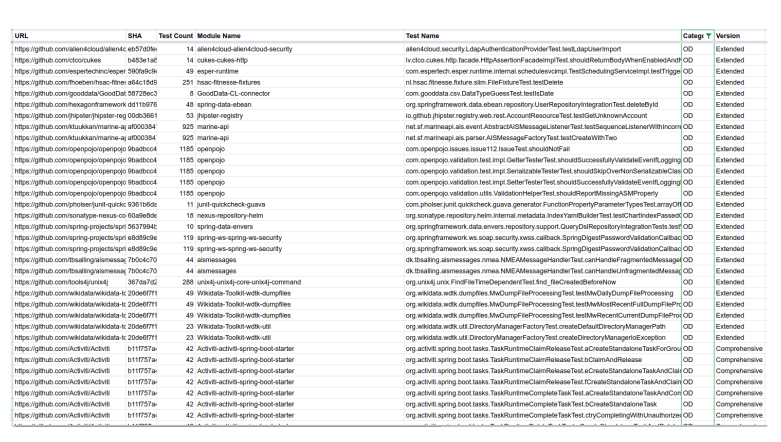
\includegraphics[width=1\textwidth]{3.1}
	\caption{\emph{Parte del dataset di IDFlakies}}
	\label{fig:datasetRilasciato}
\end{figure}
Questo framework recupera il link e lo sha di ogni repository e crea
un’immagine Docker\footnote{Docker è un progetto open-source che automatizza il deployment di applicazioni all'interno di contenitori software, fornendo un'astrazione aggiuntiva grazie alla virtualizzazione a livello di sistema operativo di Linux.}. Una volta scaricato il progetto, prova ad eseguire una delle configurazioni sopra descritte su una delle immagini Docker appena create. È possibile inoltre settare \emph{iDFlakies} per permettergli di eseguire tutte le
configurazioni in maniera consequenziale, oppure scegliere solo alcune di queste configurazioni. 

Nel momento in cui viene riscontrato un “fail” in un particolare test case in una di queste cinque configurazioni, il tool riesegue la classe di test con lo stesso ordine. Se nella seconda esecuzione il metodo mostra ancora un “fail” allora
viene classificato come OD (\textbf{O}rder \textbf{D}ependent); in caso contrario, il caso di test
viene classificato come NO (\textbf{N}o \textbf{O}rder Dependent).

Nel dataset considerato è presente anche la colonna “Version”, tale voce può assumere due possibili valori: “Comprehensive” ed “Extended”. Con l’etichetta “Comprehensive” viene identificato un test su cui sono state utilizzate tutte e cinque
le configurazioni sviluppate al fine di individuare il \emph{flaky test}, mentre con l’etichetta “Extended” si indica che su quello specifico caso di test è stata utilizzata
unicamente la configurazione “\emph{random-class-method}” (descritta precedentemente).

Tale scelta è stata fatta poiché in alcuni casi l’esecuzione di tutte e cinque le configurazioni risultava estremamente lenta e costosa.

Per costruire il nuovo dataset si è deciso di estrarre circa duecento righe del dataset di \textbf{iDFlakies}. L’estrazione è stata fatta selezionando soltanto le linee etichettate come “NO”. Di queste duecento righe sono state successivamente
scartate tutte quelle che facevano riferimento al progetto “\textbf{Apache Hadoop}” poiché la build di tale progetto impiegava svariate ore per terminare. Si è quindi deciso di lavorare sui restanti centosessanta sei metodi.

La prima operazione effettuata sul dataset originale è stata quella di eliminare le colonne “Test Count”, “Category” e “Version”, poiché ritenute poco utili ai fini dello studio. La procedura è stata effettuata manualmente con l’aiuto di un plugin di “Visual Studio Code”. Alla fine di questa fase è stato quindi ottenuto un csv con i seguenti attributi:
\begin{itemize}
	\item URL;
	\item SHA;
	\item Module Name;
	\item Test Name.
\end{itemize}
\subsection{Primo approccio}
La prima prova di classificazione delle root cause è stata fatta tramite
l’utilizzo dell’IDE di IntelliJ IDEA. L’IDE in questione ha la possibilità di eseguire un caso di test in diverse configurazioni. Tra le configurazioni possibili, si possono citare:
\begin{itemize}
\item \emph{Ripeti finché non fallisce}: Tale configurazione riesegue un caso di test (o una suite di test) finché non viene individuato un fallimento;
\item \emph{Ripeti N volte}: Tale configurazione ripete un caso di test (o una suite) un numero prestabilito di volte.
\end{itemize}

Sono stati quindi importati diversi progetti all’interno dell’ambiente di sviluppo e sono stati eseguiti diversi “run” per verificare manualmente la flakiness dei metodi analizzati. Tale strategia ha però evidenziato uno dei limiti di questa
ricerca, in quanto in svariati casi sono stati riscontrati problemi nell’effettuare con successo la build del sistema. Le problematiche più comuni in questa fase sono state sia legate a dipendenze non presenti (es. librerie non più supportate o mancanti) sia
a problemi di configurazione all’interno del file POM. A causa di questi problemi legati alla configurazione dei progetti si è deciso di scartare questo approccio di classificazione manuale.
\subsection{Secondo Approccio}
Dato che l’approccio precedente non aveva fornito una soluzione accettabile si è deciso di slegarsi dagli IDE e di trovare un approccio alternativo. In questo secondo approccio si è deciso di analizzare e automatizzare il processo di esecuzione dei singoli casi di test.

Per effettuare tali automatismi, sono stati creati una serie di script BASH. Di seguito vengono elencati nello specifico tutti i file che sono stati generati per la prima creazione del progetto.
\begin{itemize}
	\item ConfigFile;
	\item Input.csv;
	\item IDFlakies.sh;
	\item FirstStep.sh;
	\item SecondStep.sh;
	\item MainStep.sh.
\end{itemize}

\subsubsection{IDFlakies.sh}
Lo script “IDFlakies.sh” prende in input un file csv precedentemente
modificato (ovvero senza le colonne di “Test Count”, “Category” e “Version”) e scarica i repository indicati all’interno del file. Successivamente esegue il comando \emph{git checkout} e si allinea alla commit indicata. Esegue poi il comando \emph{mvn install -
DskipTests -fn -B}, e ricostruisce il path del “Module Name” indicato nel progetto cercando il sotto modulo più “vicino” alla classe presa in esame. Infine, le informazioni di interesse per lo studio vengono salvate all’interno di un nuovo file csv denominato “outIDFlakies.csv”. Lo script ha eseguito i passaggi sopra indicati per ogni riga presente all'interno del file “Input.csv”.
\subsubsection{FirstStep.sh}
Lo script “FirstStep.sh” legge il contenuto del file “outIDFlakies.csv” e per ogni riga esegue il comando \emph{mvn install -DskipTests -fn -B}. Tale comando viene
rieseguito anche in questa fase in quanto all’interno del dataset sono presenti alcuni progetti ripetuti, ma con sha differenti, si ha quindi bisogno di allinearsi ogni volta al branch corrente; l’output di questo comando viene salvato all’interno di un csv denominato “outFirstStep.csv”.
\subsubsection{SecondStep.sh}
Lo script “SecondStep.sh” può essere considerato il cuore del progetto. Lo script legge il contenuto del file csv “outFirstStep.csv” e successivamente per ogni repository esegue il comando (messo a disposizione da \textbf{Maven}) \emph{mvn -
Dtest=ClassName\#MethodName test}.
Tale comando permette l’esecuzione di un singolo caso di test isolandolo dai restanti. Lo script analizza l’output generato e in 
base al risultato del test aumenta il contatore dei pass o dei fail di una unità. Questa
operazione viene eseguita N volte per poi salvare all’interno di un csv denotato “finalCSV.csv” il risultato finale.
\subsubsection{MainStep.sh}
È stato infine creato uno script per eseguire in modo sequenziale gli step sopra descritti. Tale script fa uso di un file di configurazione chiamato “ConfigFile” dove al suo interno è stato possibile configurare il numero delle ripetizioni ed il nome dei
file che dovevano essere generati alla fine di ogni fase.
\subsection{Ottimizzazione degli script}
Una volta terminata la prima versione del progetto, quest'ultimo è stato effettivamente testato all’interno di un ambiente reale. In questa fase sono emerse diverse criticità dovute soprattutto alla lentezza di esecuzione della build per alcune repository presenti; inoltre, si è notato che le informazioni di cui si è effettivamente
tenuto traccia non erano sufficienti per permettere un’analisi dettagliata dei \emph{flaky test} riscontrati. Si è quindi deciso di creare una nuova versione per sopperire a tali mancanze.
\subsubsection{IDFlakies.sh 2.0}
L’unica modifica effettuata sullo script di “IDFlakies” è stata quella di aggiungere il nome del repository in una delle colonne di output del file “outputIDFlakies.csv”. Tale informazione infatti viene spesso utilizzata anche nelle fasi successive, ma nella prima versione veniva ricavato ogni volta.

Di seguito è mostrato il codice dello script “IDFlakies.sh”.

\lstinputlisting{code/IDFlakies.sh}
L’output di questo script consiste in un file csv (“outputIDFlakies.csv”) con la seguente intestazione:
\begin{itemize}
	\item Name Repository;
	\item Link Repository;
	\item Sha della commit;
	\item Module Name;
	\item Class Name;
	\item Method Name.
\end{itemize}

In figura \ref{fig:outputIDFlakies} è possibile osservare un esempio completo dell’output generato dallo script “IDFlakies.sh”.
\newpage
\begin{figure}[h]
	\centering
	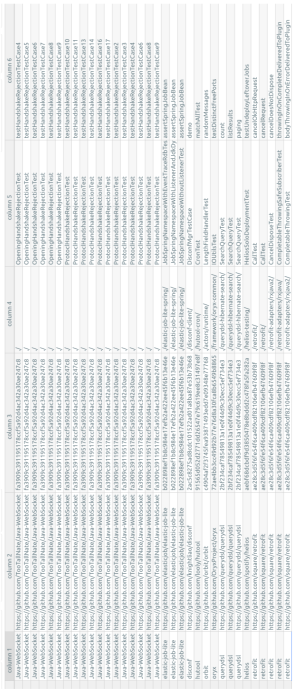
\includegraphics[width=1\textwidth]{3.2}
	\caption{\emph{Esempio di output generato da IDFlakies.sh}}
	\label{fig:outputIDFlakies}
\end{figure}
\subsubsection{FirstStep.sh 2.0}
Per quanto riguarda “FirstStep.sh”, è stato nuovamente sviluppato il
meccanismo per eseguire la build del progetto. In questa nuova versione dello script la build del progetto viene eseguita solo nel momento in cui il repository non è posizionata sul branch di nostro interesse. Per individuare l’attuale branch, viene quindi effettuato il comando di git checkout seguito dallo sha individuato nel file di
input. Se il comando dà esito positivo (ovvero viene segnalato il posizionamento su un nuovo branch), allora viene nuovamente eseguito il comando di mvn install, altrimenti, se dà esito negativo (ovvero, viene segnalato di essere già sul branch desiderato), non viene effettuata la build del progetto. Tale controllo ha permesso
di ottimizzare i tempi di esecuzione in quanto viene effettuata la build del sistema solo in caso di effettiva necessità. Infine, si è deciso di salvare all’interno del file csv di output anche il risultato della build del progetto al fine di rendere disponibile
tale informazione per analisi future.

Di seguito è mostrato il codice per effettuare le operazioni descritte precedentemente.
\lstinputlisting{code/FirstStep.sh}

Il file csv creato da questo script conterrà le seguenti informazioni:
\begin{itemize}
	\item Name Repository;
	\item Link Repository;
	\item Sha della commit;
	\item Build result.
\end{itemize}

La figura \ref{fig:outFirstStep} mostra parte del csv generato in output dal file “outFirstStep.sh”.
\newpage
\begin{figure}[h]
	\centering
	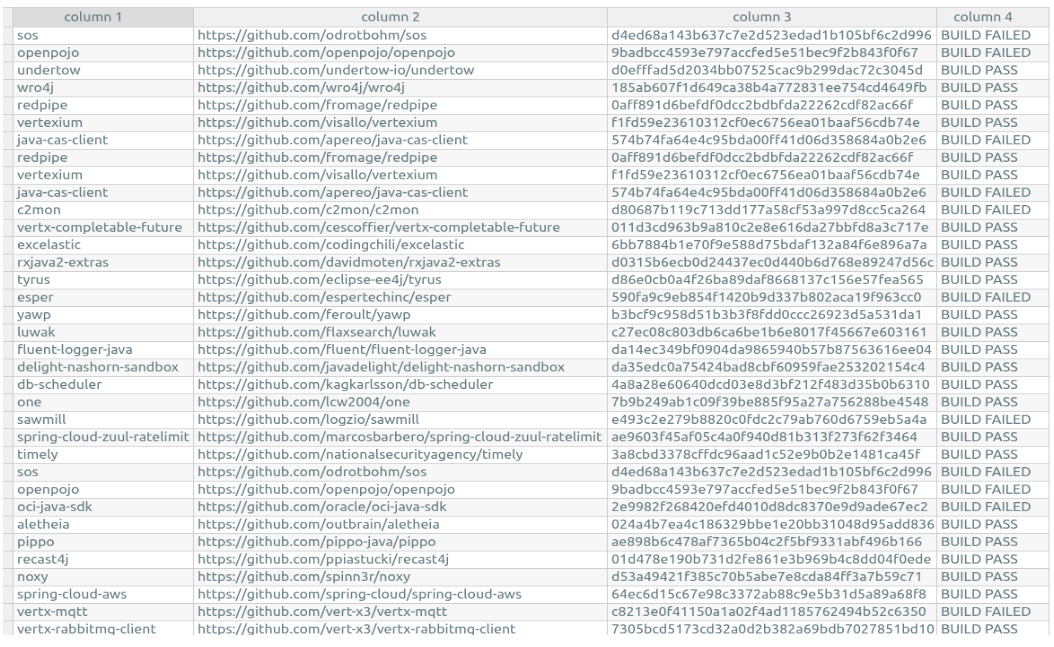
\includegraphics[width=\textwidth]{3.3}
	\caption{\emph{File creato da OutFirstStep.sh}}
	\label{fig:outFirstStep}
\end{figure}
\subsubsection{SecondStep.sh 2.0}
Per ottenere maggiori dettagli dallo script “SecondStep.sh”, si è deciso di generare un file csv intermedio per ogni metodo analizzato. Tale file contiene al suo interno le informazioni sulle N iterazioni eseguite su quel determinato caso di test. Inoltre, si è deciso di salvare su un file di log lo stato della macchina prima e
dopo l’esecuzione del metodo ed il tempo di inizio e quello di fine per ogni esecuzione effettuata, come meglio dettagliato di seguito. Tali metodi hanno permesso di ottenere dei dettagli aggiuntivi che potrebbero servire per una futura analisi. Le informazioni salvate in questo csv intermedio sono:
\begin{itemize}
	\item Name Repository;
	\item Link Repository;
	\item Sha della commit;
	\item Module Name;
	\item Class Name;
	\item Method Name;
	\item Result dell’esecuzione;
	\item Data di inizio esecuzione;
	\item Data di fine esecuzione.
\end{itemize}

La figura \ref{fig:csvIntermedio} mostra un esempio di file csv intermedio. Le informazioni raccolte nel csv intermedio sono state poi riassunte in un csv finale in cui in ogni riga vengono riportate le informazioni sul totale delle iterazioni, sul numero di successi e numero di fallimenti per quel determinato caso di test. In figura \ref{fig:csvFinale} viene riportata un estratto del csv finale generato.
\newpage
\begin{figure}[h]
	\centering
	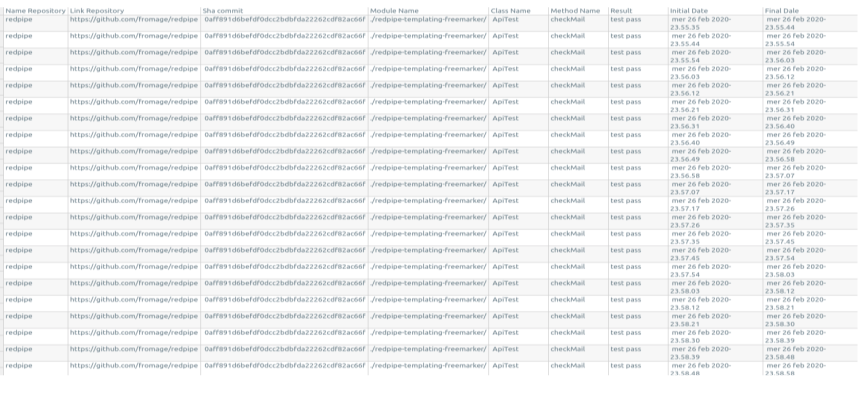
\includegraphics[width=1\textwidth]{3.4}
	\caption{\emph{Esempio del csv intermedio}}
	\label{fig:csvIntermedio}
\end{figure}
\begin{figure}[h]
	\centering
	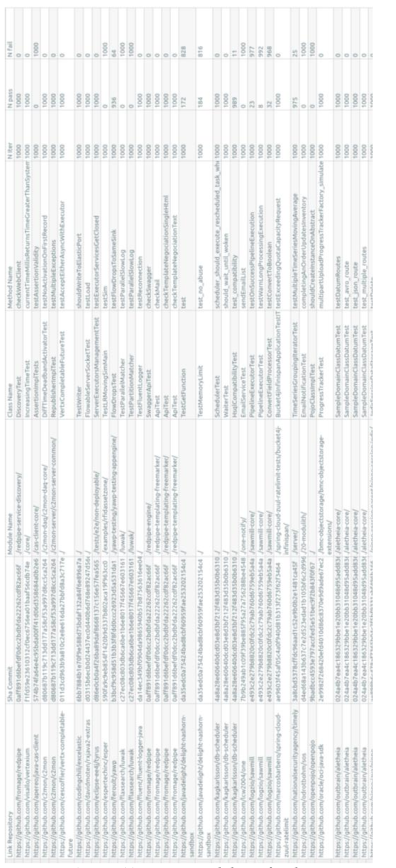
\includegraphics[width=1\textwidth]{3.5}
	\caption{\emph{Esempio del csv finale}}
	\label{fig:csvFinale}
\end{figure}

Di seguito è riportato il codice dello script “secondStep.sh”.
\lstinputlisting{code/SecondStep.sh}

Com’è possibile notare, la funzione \emph{searchFlaky()} si posiziona all’interno del module name indicato nel file csv ed effettua le seguenti operazioni:
\begin{enumerate}
	\item Salva all’interno della variabile timestampInitial il \emph{timestamp} attuale e all’interno della variabile \emph{timestampInitialDate} il timestamp convertito nel
	formato “Date”;
	\item Salva all’interno della variabile stateMachineInitial lo stato attuale della macchina prima dell’esecuzione del test, ottenuto con il comando \emph{vmstat -t};
	\item Esegue il comando \emph{mvn -Dtest=\$concatName test} e salva all’interno di un file di log il risultato;
	\item Riesegue il comando \emph{vmstat -t} per tener traccia dello stato della macchina dopo l’esecuzione del test;
	\item Calcola il nuovo timestamp di fine esecuzione e lo salva nella variabile	\emph{timeStampFinal};
	\item Controlla l’output del comando \emph{mvn -Dtest} per verificare il risultato dell’esecuzione;
	\item Se all’interno dell’output è presente la stringa “\emph{BUILD SUCCESS}” allora verrà incrementato il contatore della variabile \emph{PASSTEST} di una unità, altrimenti verrà incrementato di un’unità il contatore \emph{FAILTEST};
	\item Alla fine di ogni esecuzione vengono salvate le informazioni sul nome e il
	link del repository, lo \emph{sha} della commit, il nome della classe, il nome del metodo, il risultato ottenuto in quella iterazione ed infine il timestamp iniziale e finale entrambi convertiti in formato “Date”.
\end{enumerate}

Una volta terminata la funzione \emph{searchFlaky} viene creato un csv riassuntivo di tutte le varie iterazioni in cui sono riportate le informazioni sul numero totale di test che hanno avuto successo ed il numero totale di test che hanno avuto un fallimento come risultato.
\subsection{Esecuzione degli script su metodi OD}
Sono stati successivamente provati gli script anche sui casi di test etichettati come OD all’interno del csv rilasciato da \textbf{iDFlakies}. Lo scopo di questo test è stato quello di verificare l’effettiva dipendenza dall’ordine di esecuzione dei metodi da loro indicati. Su ogni metodo testato, l’esperimento ha dato esito negativo
(mostrando o tutti “pass” o tutti “fail”). Tale esperimento ha effettivamente comprovato che in quei casi il flaky riscontrato dipendeva dall’ordine in cui veniva eseguito il test, pertanto verranno inseriti all’interno del dataset finale attenendosi
alla classificazione data da \textbf{iDFlakies}.
\subsection{Grafico dei dati ottenuti}
L’ultima operazione effettuata è stata la creazione di grafici per i risultati ottenuti. Per effettuare questa fase sono stati individuati i \emph{flaky test} presenti all’interno del file “finalCSV.csv” e sono stati considerati i corrispettivi file csv
intermedi; si è poi andati a generare i grafici corrispondenti. Per effettuare questa fase è stato creato uno script Python per caricare i dati all’interno di un database e successivamente è stato utilizzato un tool per visualizzarli.
\subsubsection{Creazione dello script}
Lo script Python è stato suddiviso in due moduli. Il primo modulo legge tutto
il contenuto di una directory e genera in output una lista contenente tutti i file in formato csv presenti all’interno. Successivamente tramite un’apposita libreria i dati
sono stati manipolati (es. sostituendo la dicitura: “test pass” con il valore 1 e “test fail” con il valore 0) e poi sono stati passati al modulo denominato “load\_data\_influxDB”. Tale metodo sfruttando le API di InfluxDB carica i dati all’interno del database.
\subsubsection{InfluxDB e Chronograf}
Per l'immagazzinamento dei dati è stato individuato il database “InfluxDB”. Tale database è particolarmente indicato nel momento in cui bisogna rappresentare dati temporali. Nello scegliere il tool da adoperare per graficare i dati
si è optato per “\textbf{Chronograf}” in quanto è un tool sviluppato dalla stessa software
house di InfluxDB.

Di seguito vengono mostrati alcuni dei grafici generati.

Il grafico in figura\ref{fig:AndamentoFlaky} mostra l’andamento del metodo
“\emph{runReconnectBlockingScenario2}” appartenente alla classe “\emph{Issue256Test}” del progetto “\textbf{Java-WebSocket}”.
\begin{figure}[h]
	\centering
	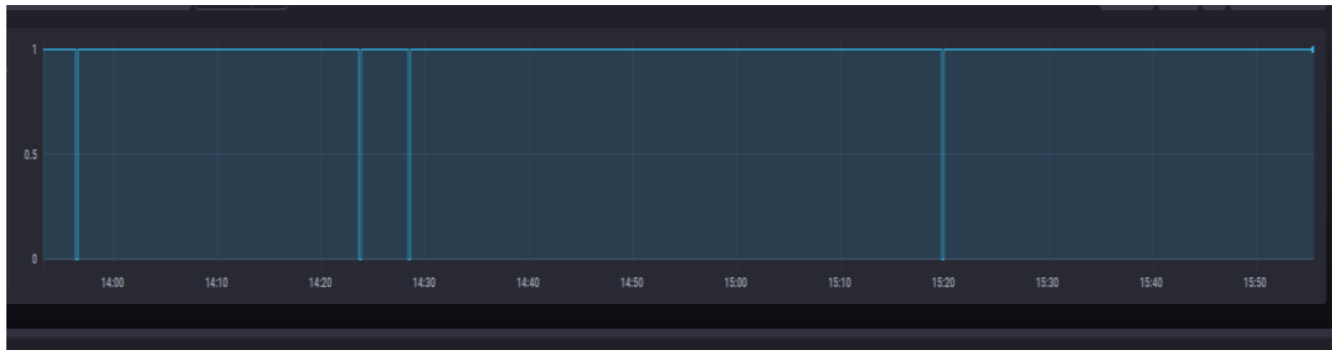
\includegraphics[width=\textwidth]{3.6}
	\caption{\emph{Andamento di uno dei metodi flaky}}
	\label{fig:AndamentoFlaky}
\end{figure}

Com’è possibile osservare dal grafico, tale metodo presenta quattro fallimenti su mille esecuzioni.\newline
Il grafico in figura \ref{fig:fallimentobulk} mostra il fallimento del metodo “\emph{testBulkClusterJoining}” appartenente alla classe “\emph{ZKTest}” del progetto “\textbf{Noxy}”.
\begin{figure}[h]
	\centering
	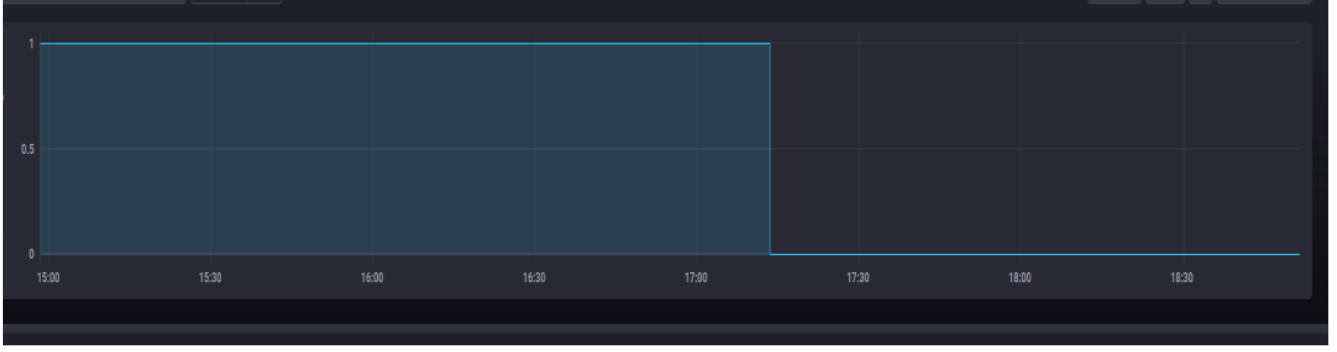
\includegraphics[width=\textwidth]{3.7}
	\caption{\emph{Andamento del metodo testBulkClusterJoining}}
	\label{fig:fallimentobulk}
\end{figure}
\newline
Il metodo preso in esame presentava una serie di successi consecutivi (152) per poi iniziare una serie di fallimenti (848). Il metodo quindi è stato ritestato ma ha dato sempre risultati simili a quello mostrato precedentemente.
L’ultimo metodo che si vuole illustrare è del progetto “timely”. Il metodo in questione è: “\emph{testMultipleTimeSeriesMovingAverage}” appartenente alla classe
“\emph{TimeSeriesGroupingIteratorTest}”. Tale metodo risulta molto interessante poiché mostra un fallimento ogni volta che scatta il 58esimo minuto di un’ora.
La figura 3.8 mostra l’esecuzione del metodo
\begin{figure}[h]
	\centering
	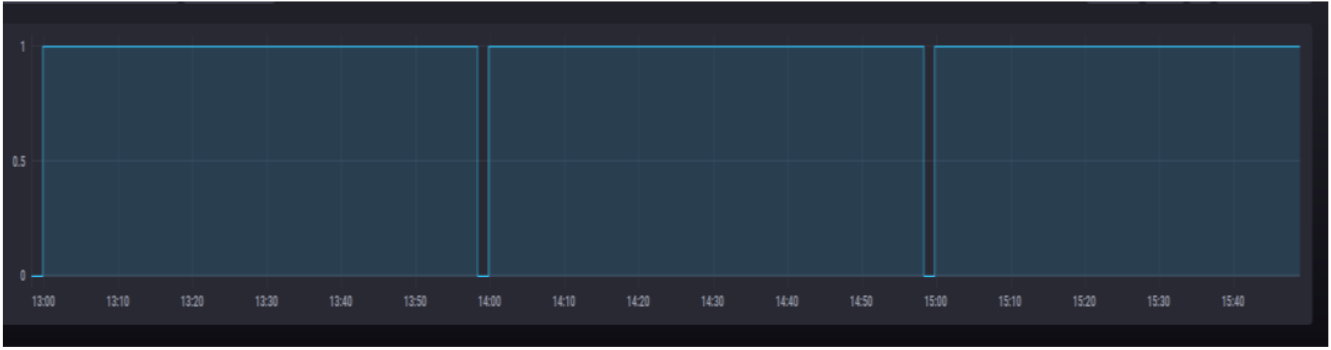
\includegraphics[width=\textwidth]{3.8}
	\caption{\emph{Andamento di testMultipleTimeSeriesMovingAverage}}
	\label{fig:patternFlaky}
\end{figure}
Per ottenere una maggiore sicurezza, si è quindi proceduto ad eseguire altre due volte il metodo sopra elencato.
Le figure \ref{fig:riesecuzione1} e \ref{fig:riesecuzione2} mostrano i risultati delle altre esecuzioni effettuate.
\begin{figure}[h]
	\centering
	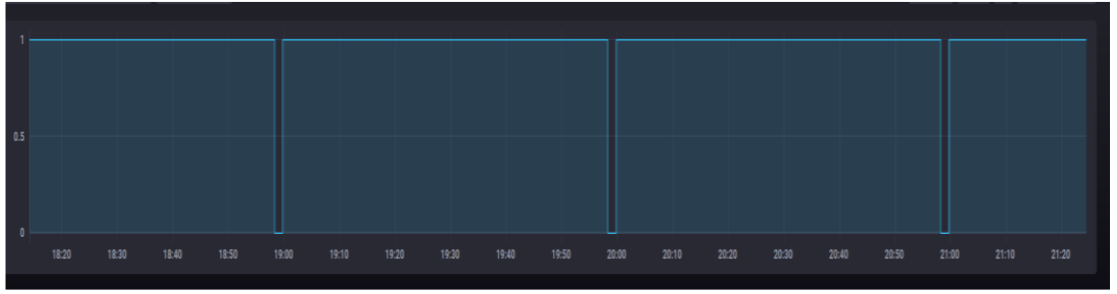
\includegraphics[width=\textwidth]{3.9}
	\caption{\emph{Seconda esecuzione del test in analisi}}
	\label{fig:riesecuzione1}
\end{figure}
\begin{figure}[h]
	\centering
	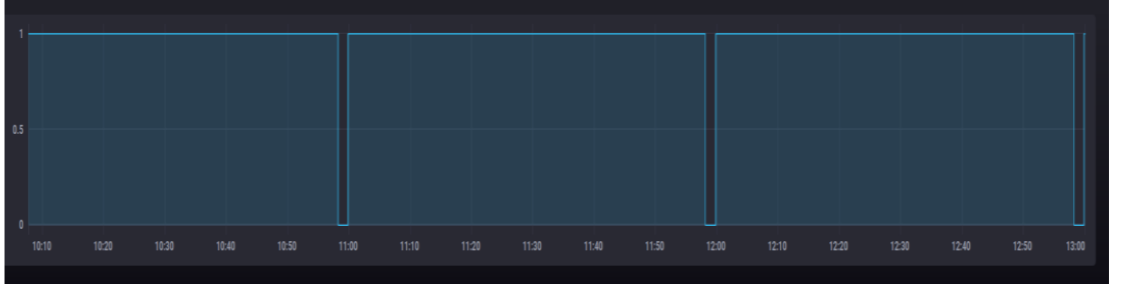
\includegraphics[width=\textwidth]{3.10}
	\caption{\emph{Terza esecuzione del test in analisi}}
	\label{fig:riesecuzione2}
\end{figure}
\newline
Possiamo quindi considerare questo tipo di flaky “deterministico” in quanto presenta un pattern ben preciso.
\subsection{Root cause più frequenti}
Sono state infine analizzate le root cause dei flaky test individuati tramite una
analisi statica del codice. Tale analisi è stata fatta sui repository con comportamenti più “stabili” (ovvero un numero bilanciato sia di “pass” che di “fail”), e sono emersi
i seguenti risultati:
\begin{itemize}
	\item 99\% Errore di Network;
	\item 1\% Multithreading.
\end{itemize}
Tali risultati andrebbero però inquadrati in contesti più ampi e con più dati a disposizione.
\subsection{Limiti della ricerca}
Durante tutta la fase di ricerca sono emersi diversi limiti, alcuni dei quali sono stati trattati precedentemente, altri invece vengono presentati in questa sezione.
\begin{itemize}
\item Lentezza dell’esecuzione della build: In alcuni casi sono state analizzati progetti la cui build ha impiegato oltre due/tre ore per terminare. Tale problematica è sintomo di sistemi di building ancora non adeguatamente efficienti;
\item Lentezza nell’eseguire un singolo caso di test: In alcuni casi sono stati impiegati svariati minuti per eseguire un singolo caso di test; da una indagine effettuata, il sistema di build di Maven riconfigura parte dell’ambiente ad ogni singola esecuzione. Tale riconfigurazione può impiegare anche diversi minuti;
\item Limiti hardware: Gli esperimenti sono stati eseguiti su una macchina Ubuntu 16.04 4GB di RAM 2. Intel Core i3-2100 CPU 3.10GHzx4;
\item Sha non validi: In alcuni casi non c’è stata la possibilità di eseguire l’allineamento sul branch indicato dal dataset in quanto è stato restituito il seguente errore: “reference is not a tree” nel momento in cui è stato eseguito il comando “git checkout”.
\end{itemize}
